% Chapter Template

\chapter{System Design and Development} % Main chapter title

\label{Chapter4} % Change X to a consecutive number; for referencing this chapter elsewhere, use \ref{ChapterX}

\lhead{Chapter 4. \emph{System Design and Development}} % Change X to a consecutive number; this is for the header on each page - perhaps a shortened title

%----------------------------------------------------------------------------------------

\section{Introduction}

This chapter will the requirements that the system must fulfil, outline the challenges involved and highlight the key technologies that I will be using.


%----------------------------------------------------------------------------------------

\section{Cross-Platform}

One of the main requirements is running on multiple devices so that the usability of the service is maximised. Although this project will only target the Android platform, it will be designed such that it can be adapted to also run on iOS.

For the sake of simplicity and given the time requirements, this project will also aim to implement the server and client in the same programming language.

\subsection{Mono and Xamarin}

Mono is an open source implementation of C\# that is cross-platform. This allows development of C\# code that can run on Windows, Linux and Mac.

Xamarin is a mobile app development framework built on Mono, targeting the Android, iOS, Windows Phone and Mac platforms. Because Xamarin is written in C\#, it can integrate easily with the Windows SDK for the development of Windows Desktop Applications. This allows business layer logic to be shared across the different platform implementations, essentially having one main codebase rather than one per platform.

\begin{figure}[htbp]
	\centering
		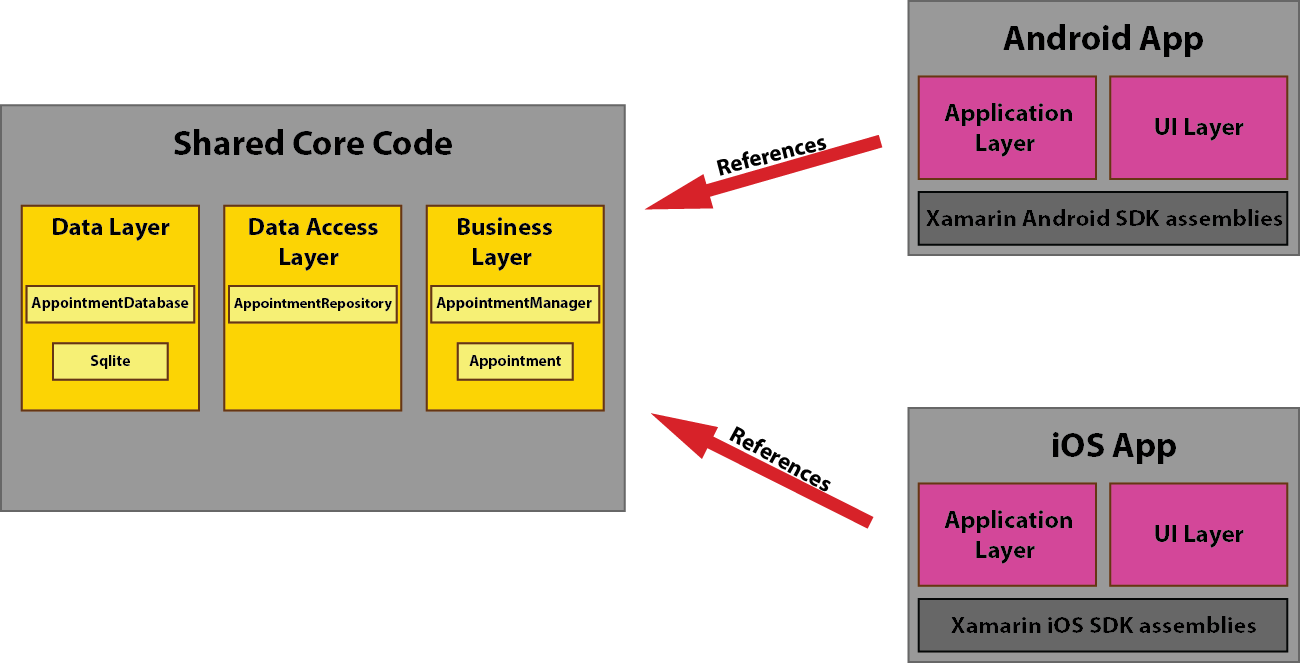
\includegraphics[width=\textwidth,height=\textheight,keepaspectratio]{Figures/AppOverview.png}
		\rule{35em}{0.5pt}
\end{figure}

\subsection{Conclusion} 

The server application will be written in C\# and compiled using Mono, allowing it to run on either Windows or Linux server machines. The Android App will also be written in C\# using the Xamarin framework, allowing the codebase to be easily integrated with future platforms.

%----------------------------------------------------------------------------------------

\section{Communication}

The system requires two types of communication based on the requirements, urgent and direct. It is very important to differentiate between these two when targeting mobile devices, due to the following issues:
\begin{itemize}
	\item Bandwidth is limited
	\item Devices aren't always online
	\item Connections are unreliable
	\item Constant communication can cause excessive power consumption
\end{itemize}

Due to these issues, a constant connection to a remote server is not possible for long periods of time. This means that the communication must be separated into two separate components, each being useful for different scenarios.

\subsection{Push Communication}

Notification messages, also known as push notifications, are a way of sending a short notification message to a device. This is useful for sending urgent messages when the application is not being used, prompting the user for input.

There are however, limitations of this type of communication:

\begin{itemize}
	\item Only small messages are allowed to be sent
	\item The server does not know when the message has been received
	\item Server to client messages only
\end{itemize}

Push communication can be seen as a 'answering machine service'. The server leaves a short message for the device to be received at some point in the future. If the device is offline, it will receive the message as soon as it comes online again, making it a good system for unreliable connections.

Push notifications should be kept short and only contain enough data to notify the application that it needs to connect to the server for more information.

Due to these limitations, the system will only use push notifications for the following scenarios:

\begin{itemize}
	\item A sooner appointment is available for the patient
	\item An appointment has been cancelled and/or needs rescheduling
	\item Information about an appointment has been changed
\end{itemize}

\subsubsection{Google Cloud Messaging (Android)}

Google Cloud Messaging is the Android service for sending push notifications. It has a message limit of 4kb and requires the Google Play Store to function. It is a free service, however it has a daily limitation on how many notifications can be sent from a single application.

\begin{figure}[htbp]
	\centering
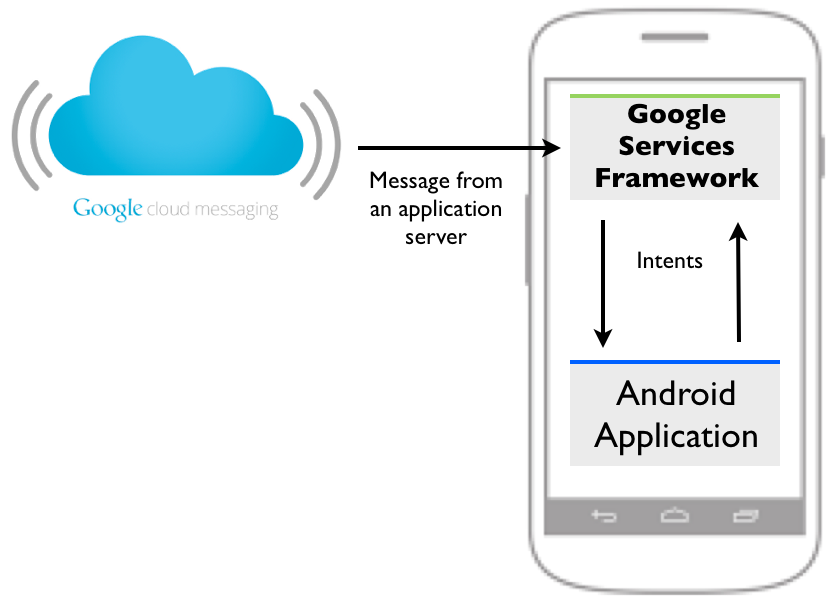
\includegraphics[width=10cm,height=10cm,keepaspectratio]{Figures/PushNote.png}
		\rule{35em}{0.5pt}
	\caption[Google Cloud Messaging]{Google Cloud Messaging}
	\label{fig:PushNote}
\end{figure}

By using this service, messages are queued and sent to the device as soon as it is available, prompting the user of some kind of notification relating to the application.

\subsubsection{Apple Push Notifications Gateway (iOS)}

Apple also have a push notification service. It has a message limit of just 256 bytes.

\subsection{Direct Communication}

After a notification has been received, or simply through using the applications features, the device will require direct communication with the server. It will require communication to:

\begin{itemize}
	\item Create or Reschedule an appointment.
	\item Request information about an appointment
	\item Request reminders about an appointment
	\item Requesting the database encryption key
\end{itemize}

\subsubsection{RESTful Web Services}

To be written.

\begin{figure}[htbp]
	\centering
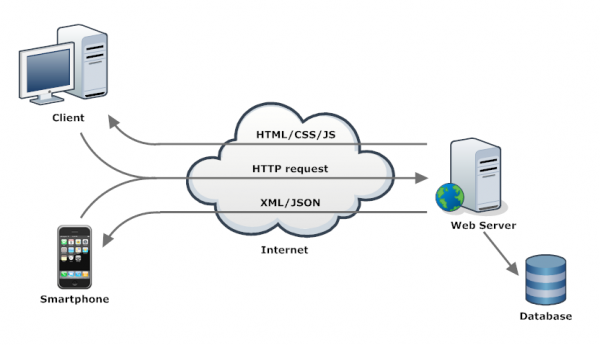
\includegraphics[width=10cm,height=10cm,keepaspectratio]{Figures/rest.png}
		\rule{35em}{0.5pt}
	\caption[RESTful Web Services cross-platform communication]{RESTful Web Services cross-platform communication}
	\label{fig:rest}
\end{figure}


%----------------------------------------------------------------------------------------

\section{Data}

Appointment data will be cached on the mobile so that communication is minimised. Data will be stored in an sqlite database because it is built into both the Android and iOS operating systems, making it available on all target devices.

\subsection{Security}

Data security is an issue because we are dealing with sensitive patient data. Because of this, the database must be encrypted.

%----------------------------------------------------------------------------------------
